\usepackage[
  paper=a4paper,
  layout=a4paper,
  top=25mm,
  bottom=22mm,
  left=25mm,
  right=25mm,
  marginparsep=5mm,
  marginparwidth=20mm,
  head=7.5mm,
  foot=8mm
  ]{geometry}

\usepackage{fontspec}
\defaultfontfeatures{Mapping=tex-text}
\setmainfont{Inter}[Path = /home/tobias/Dokument/r2book/resources/Inter/static/,Extension = .ttf,UprightFont = *-Regular,FontFace={ul}{n}{Font=*-Light},FontFace={l}{n}{Font=*-Light},FontFace={m}{n}{Font=*-Regular},FontFace={b}{n}{Font=*-Medium},]
\DeclareRobustCommand{\ulseries}{\fontseries{ul}\selectfont}
\DeclareRobustCommand{\lseries}{\fontseries{l}\selectfont}
\DeclareRobustCommand{\mseries}{\fontseries{m}\selectfont}
\DeclareRobustCommand{\mbseries}{\fontseries{mb}\selectfont}
\DeclareRobustCommand{\bseries}{\fontseries{b}\selectfont}
\DeclareRobustCommand{\ebseries}{\fontseries{eb}\selectfont}
\DeclareTextFontCommand{\textul}{\ulseries}
\DeclareTextFontCommand{\textl}{\lseries}
\DeclareTextFontCommand{\textm}{\mseries}
\DeclareTextFontCommand{\textmb}{\mbseries}
\DeclareTextFontCommand{\textb}{\bseries}
\DeclareTextFontCommand{\texteb}{\ebseries}
\setsansfont{SpecialElite}[Path = /home/tobias/Dokument/r2book/resources/SpecialElite/,Extension = .ttf,UprightFont = *-Regular]
\newfontfamily{\hwfamily}{Tillana}[Path = /home/tobias/Dokument/r2book/resources/Tillana/,Extension = .ttf, UprightFont = *-Regular]

\linespread{1.075}
\parskip = .5\baselineskip

\makeatletter
\def\@maketitle{%
  \newpage
  \null
  \vskip -\topskip%
  \begin{center}%
    {\strut\LARGE\sffamily \@title \par}%
    \vskip 2\baselineskip%
  \end{center}}
\makeatother

\usepackage{lastpage}

\newcommand\thexex{0}
\newcommand\xex[1]{\renewcommand\thexex{#1}}

% https://github.com/rstudio/bookdown/issues/677
\let\paragraph\oldparagraph
\let\subparagraph\oldsubparagraph

\usepackage{titlesec}
\titlespacing{\section}{0pt}{1.5\baselineskip}{.5\baselineskip}
\titlespacing{\subsection}{0pt}{1\baselineskip}{.25\baselineskip} %.5
\titlespacing{\subsubsection}{0pt}{1\baselineskip}{.25\baselineskip} %.25

\newpagestyle{respekt}[\large\sffamily]{
\sethead{}{}{\hbox{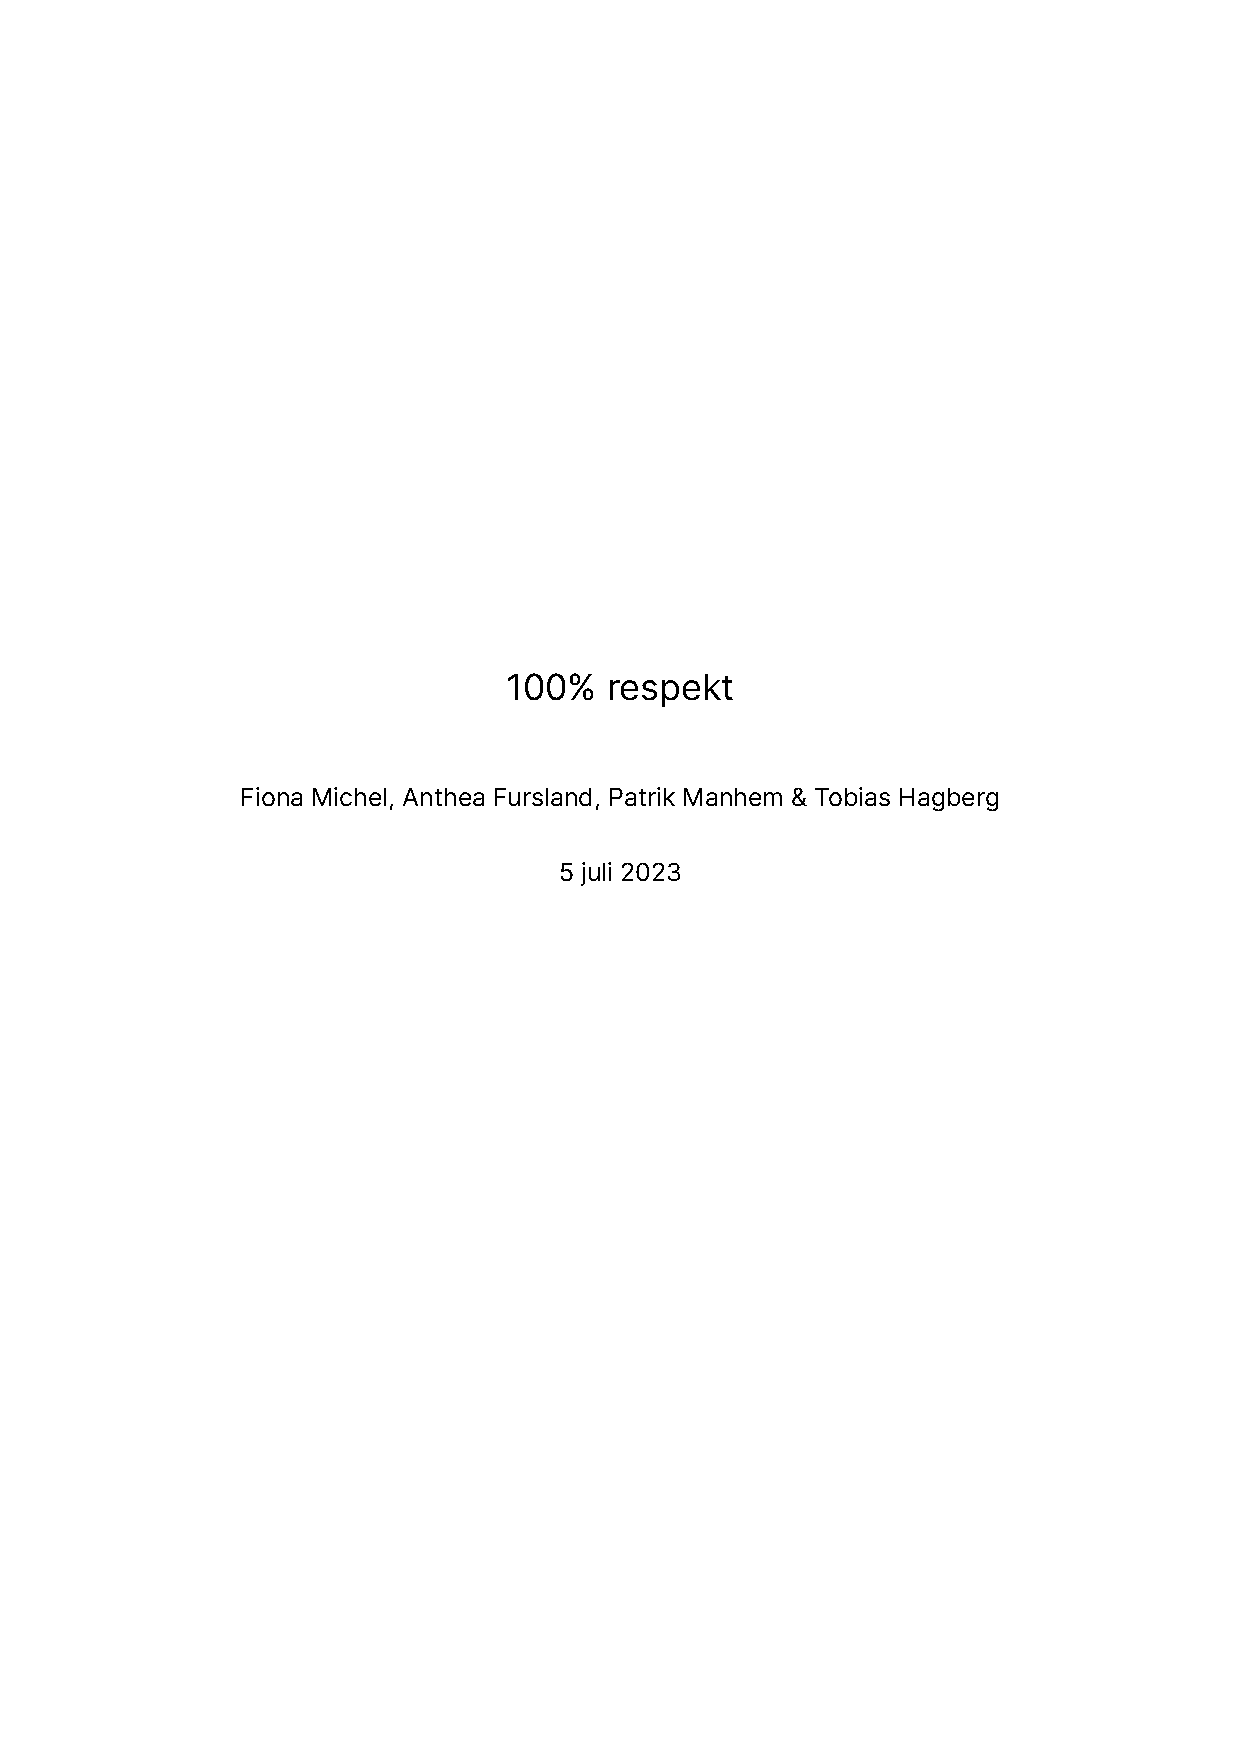
\includegraphics[width=13mm]{/home/tobias/Dokument/r2book/sites/respekt/media/image/100respekt.pdf}}}
\setfoot{\rmfamily\small\thepage/\pageref*{LastPage}}{}{}
}

\newpagestyle{respektExample}[\large\sffamily]{
\sethead{\if 0\thexex\else
\begin{tikzpicture}[]\node[rotate=5] at (0,0) {\hwfamily\Large\color{MidnightBlue}Exempel};\end{tikzpicture}\fi}{}{\hbox{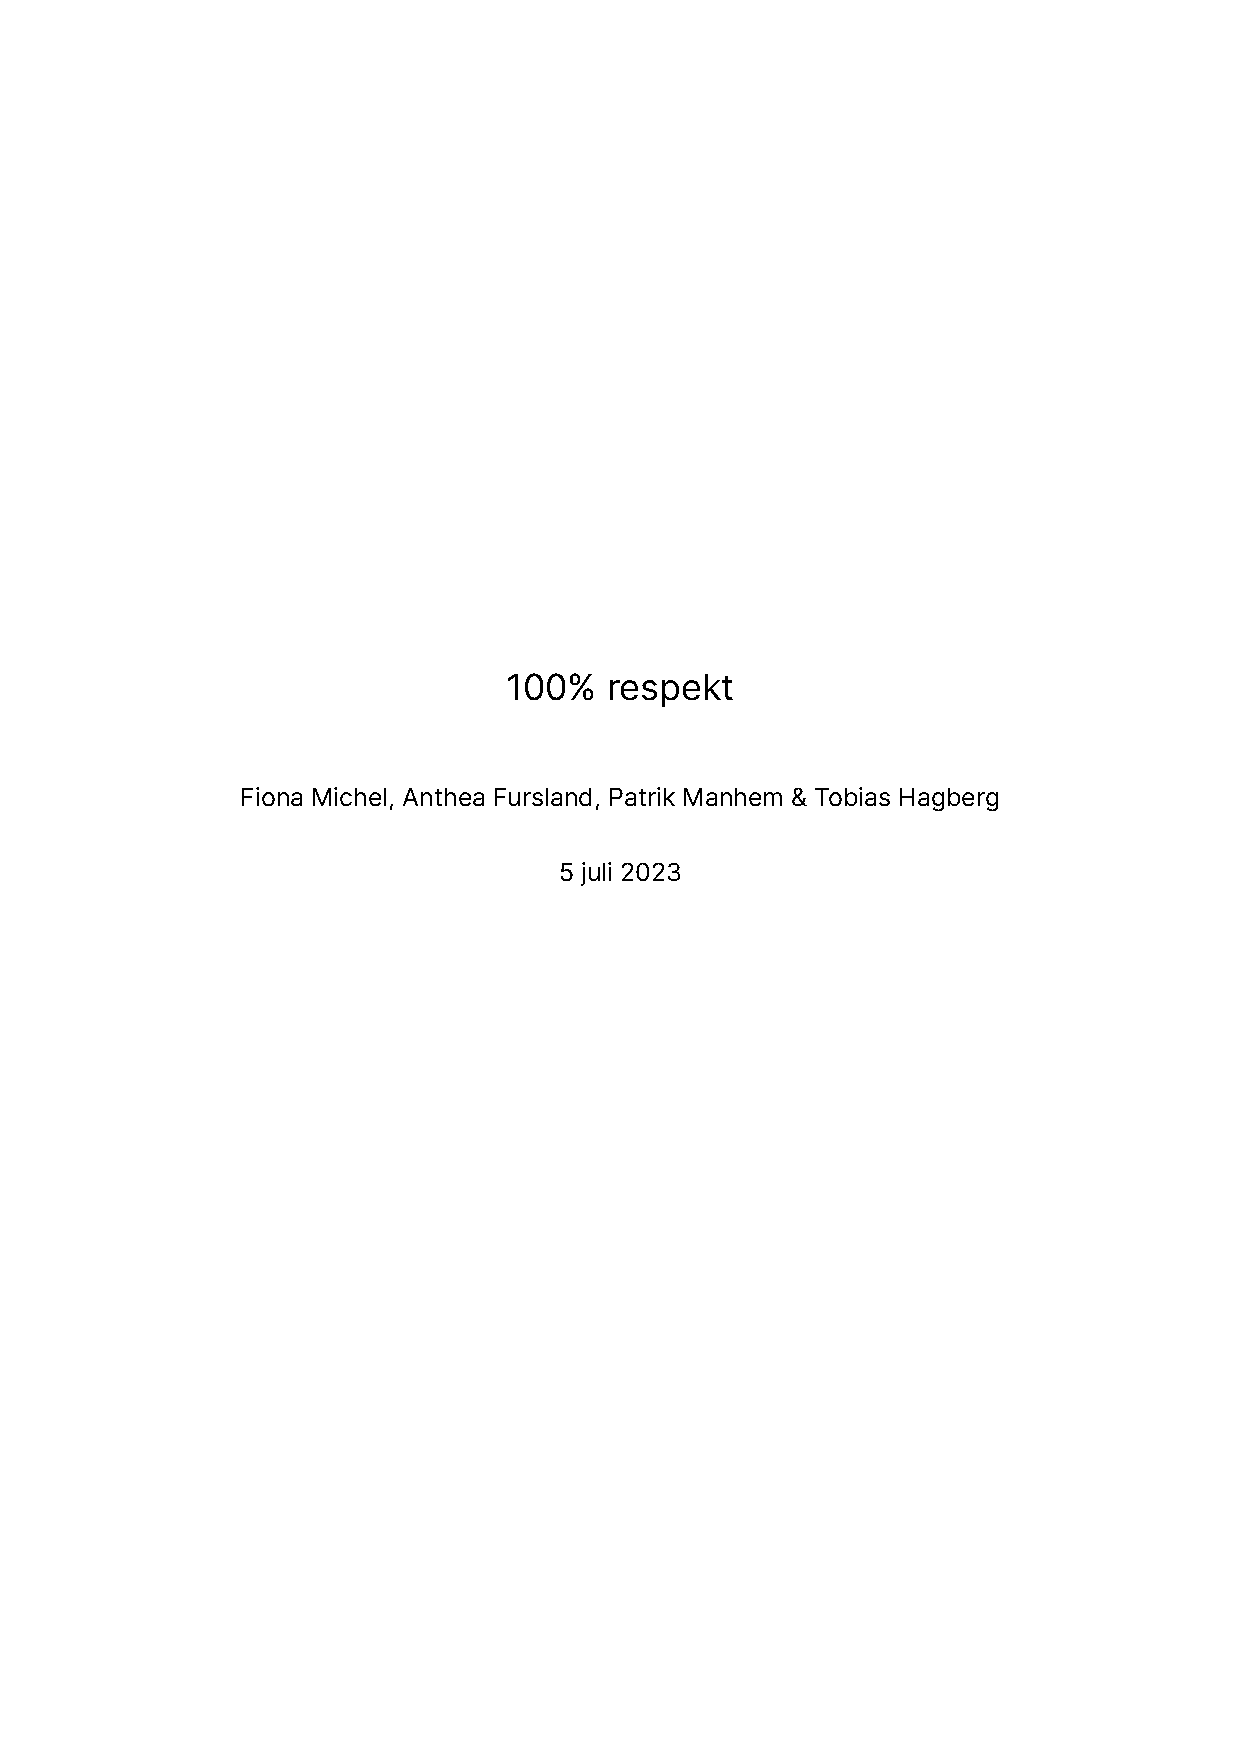
\includegraphics[width=13mm]{/home/tobias/Dokument/r2book/sites/respekt/media/image/100respekt.pdf}}}
\setfoot{\rmfamily\small\thepage/\pageref*{LastPage}}{}{}
}

\newpagestyle{respektTurn}[\large\sffamily]{
\sethead{\if 0\thexex\else
\begin{tikzpicture}[]\node[rotate=5] at (0,0) {\hwfamily\Large\color{MidnightBlue}Exempel};\end{tikzpicture}\fi}{}{\hbox{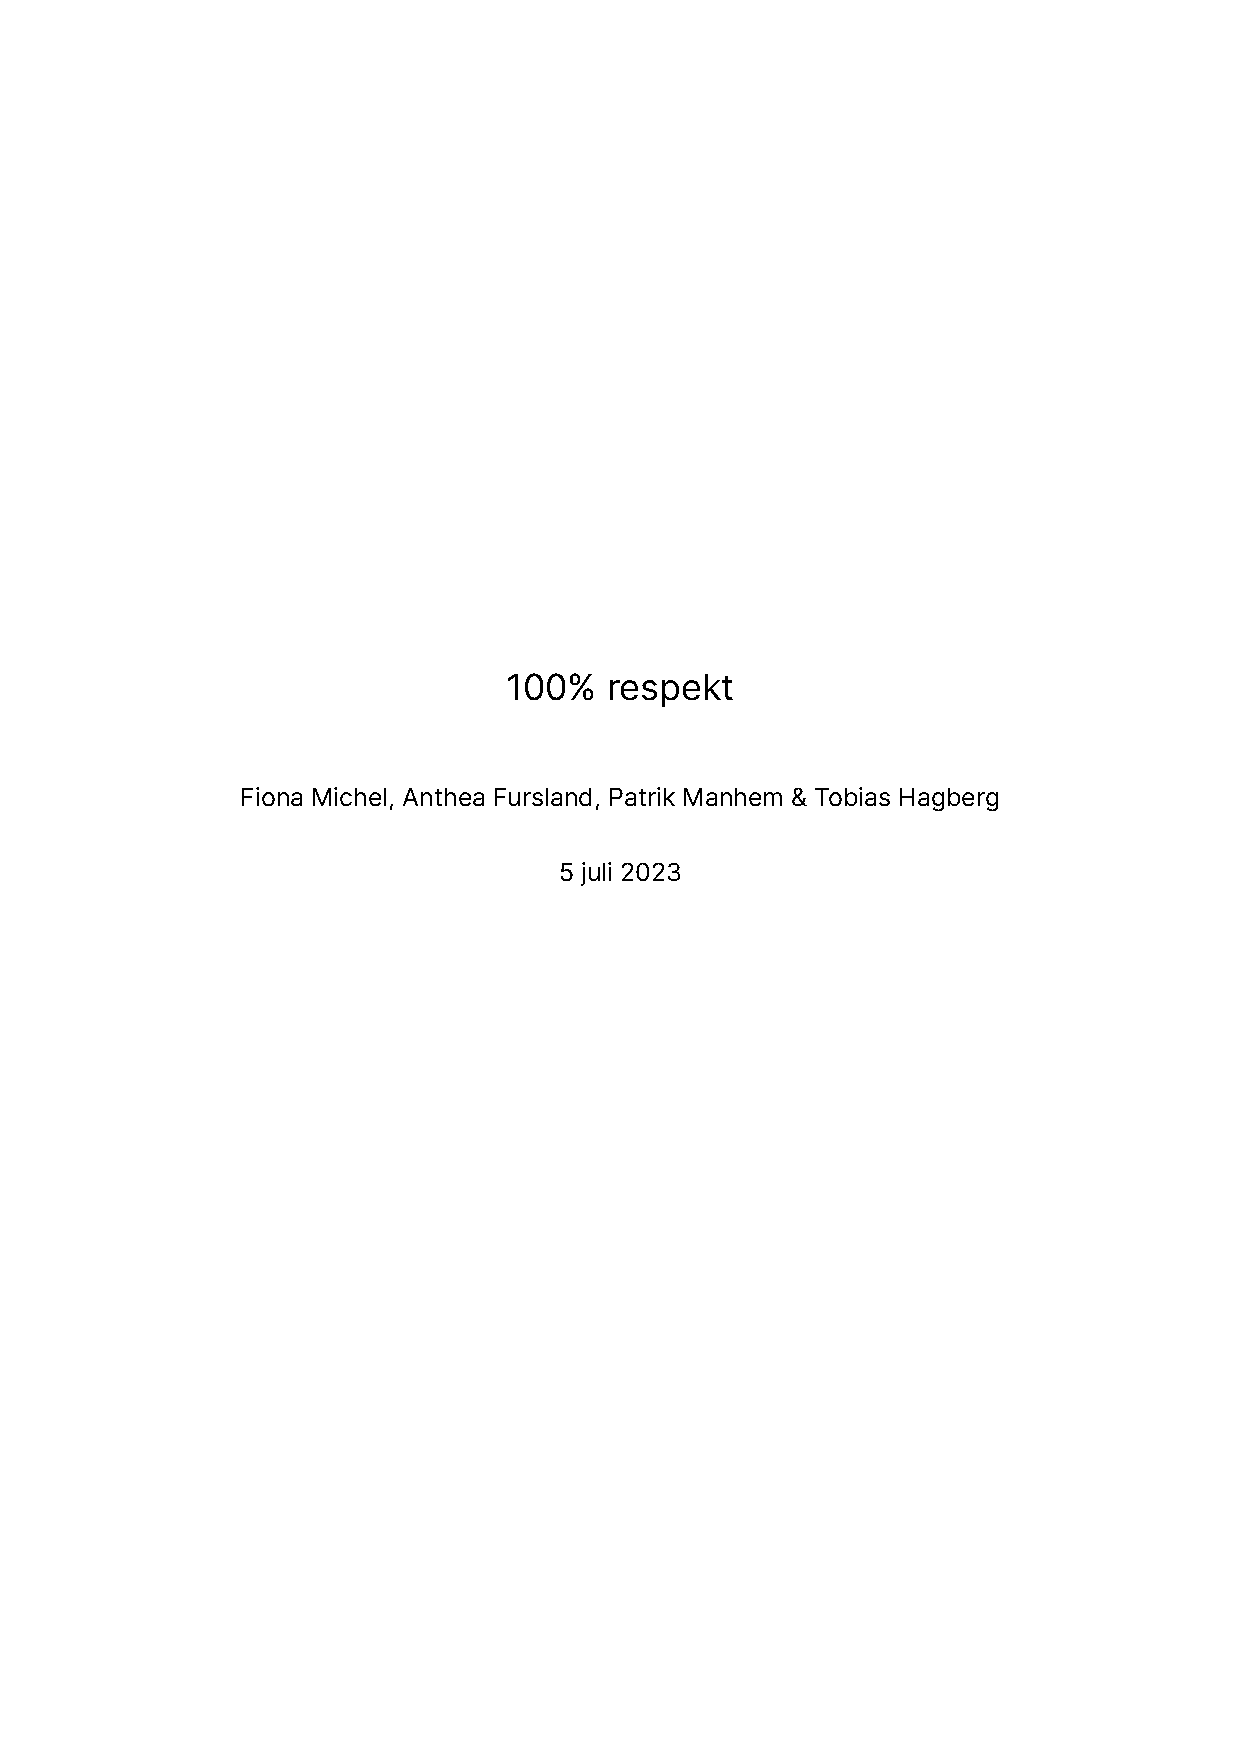
\includegraphics[width=13mm]{/home/tobias/Dokument/r2book/sites/respekt/media/image/100respekt.pdf}}}
\setfoot{\rmfamily\small\thepage/\pageref*{LastPage}}{}{\rmfamily\small Arbetsbladet fortsätter på nästa sida}
}

\newcommand\xturn{\thispagestyle{respektTurn}\pagebreak}
\pagestyle{respekt}

\usepackage{ragged2e,pgf,tikz,pgffor}
\newcommand\xtikzsquare{\begin{tikzpicture}\draw (0,0) node[minimum size=9mm,draw] {};\end{tikzpicture}}
\newcommand\xtikztick{\begin{tikzpicture}\draw (0,0) node[minimum size=1ex,draw] {};\end{tikzpicture}}
\newcommand\xtikztickz[1]{\begin{tikzpicture}\draw (0,0) node[minimum size=#1,draw] {};\end{tikzpicture}}

\usepackage{enumitem}

\newcommand{\xvskip}{\vspace{2.25\baselineskip}}
\newcommand{\xinit}{\fontsize{9.5bp}{12bp}\selectfont\thispagestyle{respekt}}
\newcommand{\fline}[1]{\parbox[b][2\baselineskip][b]{\textwidth}{\large\hwfamily\color{MidnightBlue}\if 1\thexex#1\else\fi}\par\vspace{-1\baselineskip}\begin{tikzpicture}\draw (0,0) -- (\textwidth,0);\end{tikzpicture}\par\vspace{-0.4pt}\vspace{-.25\baselineskip}}
\newcommand\xfline[3]{\vbox to 0mm{\bfseries #1}\foreach \n in {1,...,#2}{\fline{#3}}}
\newcommand\xhl[1]{#1 --}

\usepackage{marginnote}
\newcommand\xlist[2]{\marginnote{\scriptsize#1}\RaggedRight #2}

\newcommand\xpageref[1]{ (sidan \pageref{#1})}

\usepackage{calc}
\usepackage{qrcode}
\newcommand\xqr[3]{\vspace{.5\baselineskip}\par\hspace{0\baselineskip}\qrcode[height=2.75\baselineskip]{#2}\hspace{.75\baselineskip}\parbox{1\linewidth-3.5\baselineskip}{\small\href{#2}{#1\\\url{#2}}}\par\vspace{.5\baselineskip}}
\newcommand\xqrform[3]{\vspace{.5\baselineskip}\par\hspace{0\baselineskip}\qrcode[height=2.75\baselineskip]{https://100respekt.se/#2}\hspace{.75\baselineskip}\parbox{1\linewidth-3.5\baselineskip}{\small\href{https://100respekt.se/#2}{#1\\\url{https://100respekt.se/#2}}}\par\vspace{.5\baselineskip}}

\definecolor{quarto-callout-tip-color}{HTML}{73aa72}

%\newcommand\xqr[3]{\vspace{1.5\baselineskip}\hspace{3\baselineskip}\qrcode[height=3\baselineskip]{#1}\quad \parbox{.55\linewidth}{\small\href{#1}{#2\\\url{#1}}}\par}